%%%%%%%%%%%%%%%%%%%%%%%%%%%%%%%%%%%%%%%%%
% Programming/Coding Assignment
% LaTeX Template
%
% This template has been downloaded from:
% http://www.latextemplates.com
%
% Original author:
% Ted Pavlic (http://www.tedpavlic.com)
%
% Note:
% The \lipsum[#] commands throughout this template generate dummy text
% to fill the template out. These commands should all be removed when 
% writing assignment content.
%
% This template uses a Perl script as an example snippet of code, most other
% languages are also usable. Configure them in the "CODE INCLUSION 
% CONFIGURATION" section.
%
%%%%%%%%%%%%%%%%%%%%%%%%%%%%%%%%%%%%%%%%%

%----------------------------------------------------------------------------------------
%	PACKAGES AND OTHER DOCUMENT CONFIGURATIONS
%----------------------------------------------------------------------------------------

\documentclass{article}

\usepackage{fancyhdr} % Required for custom headers
\usepackage{lastpage} % Required to determine the last page for the footer
\usepackage{extramarks} % Required for headers and footers
\usepackage[usenames,dvipsnames]{color} % Required for custom colors
\usepackage{graphicx} % Required to insert images
\usepackage{subcaption}
\usepackage{listings} % Required for insertion of code
\usepackage{courier} % Required for the courier font
\usepackage{lipsum} % Used for inserting dummy 'Lorem ipsum' text into the template
\usepackage{hyperref} % Used for linking to websites
\usepackage{amsmath, amsthm, amssymb} % Required for writing equations
\usepackage{pythonhighlight} % Required for including Python code
\usepackage{siunitx} % Required for scientific notation

% Margins
\topmargin=-0.45in
\evensidemargin=0in
\oddsidemargin=0in
\textwidth=6.5in
\textheight=9.0in
\headsep=0.25in

\linespread{1.1} % Line spacing

% Set up the header and footer
\pagestyle{fancy}
\lhead{\hmwkFirstAuthorName, \hmwkSecondAuthorName} % Top left header
\chead{\hmwkClass\ (\hmwkClassTime): \hmwkTitle} % Top center head
%\rhead{\firstxmark} % Top right header
\lfoot{\lastxmark} % Bottom left footer
\cfoot{} % Bottom center footer
\rfoot{Page\ \thepage\ of\ \protect\pageref{LastPage}} % Bottom right footer
\renewcommand\headrulewidth{0.4pt} % Size of the header rule
\renewcommand\footrulewidth{0.4pt} % Size of the footer rule

\setlength\parindent{0pt} % Removes all indentation from paragraphs

%----------------------------------------------------------------------------------------
%	CODE INCLUSION CONFIGURATION
%----------------------------------------------------------------------------------------

\definecolor{MyDarkGreen}{rgb}{0.0,0.4,0.0} % This is the color used for comments
\lstloadlanguages{Perl} % Load Perl syntax for listings, for a list of other languages supported see: ftp://ftp.tex.ac.uk/tex-archive/macros/latex/contrib/listings/listings.pdf
\lstset{language=Perl, % Use Perl in this example
        frame=single, % Single frame around code
        basicstyle=\small\ttfamily, % Use small true type font
        keywordstyle=[1]\color{Blue}\bf, % Perl functions bold and blue
        keywordstyle=[2]\color{Purple}, % Perl function arguments purple
        keywordstyle=[3]\color{Blue}\underbar, % Custom functions underlined and blue
        identifierstyle=, % Nothing special about identifiers                                         
        commentstyle=\usefont{T1}{pcr}{m}{sl}\color{MyDarkGreen}\small, % Comments small dark green courier font
        stringstyle=\color{Purple}, % Strings are purple
        showstringspaces=false, % Don't put marks in string spaces
        tabsize=5, % 5 spaces per tab
        %
        % Put standard Perl functions not included in the default language here
        morekeywords={rand},
        %
        % Put Perl function parameters here
        morekeywords=[2]{on, off, interp},
        %
        % Put user defined functions here
        morekeywords=[3]{test},
       	%
        morecomment=[l][\color{Blue}]{...}, % Line continuation (...) like blue comment
        numbers=left, % Line numbers on left
        firstnumber=1, % Line numbers start with line 1
        numberstyle=\tiny\color{Blue}, % Line numbers are blue and small
        stepnumber=5 % Line numbers go in steps of 5
}

% Creates a new command to include a perl script, the first parameter is the filename of the script (without .pl), the second parameter is the caption
\newcommand{\perlscript}[2]{
\begin{itemize}
\item[]\lstinputlisting[caption=#2,label=#1]{#1.pl}
\end{itemize}
}

%----------------------------------------------------------------------------------------
%	DOCUMENT STRUCTURE COMMANDS
%	Skip this unless you know what you're doing
%----------------------------------------------------------------------------------------

% Header and footer for when a page split occurs within a problem environment
\newcommand{\enterProblemHeader}[1]{
%\nobreak\extramarks{#1}{#1 continued on next page\ldots}\nobreak
%\nobreak\extramarks{#1 (continued)}{#1 continued on next page\ldots}\nobreak
}

% Header and footer for when a page split occurs between problem environments
\newcommand{\exitProblemHeader}[1]{
%\nobreak\extramarks{#1 (continued)}{#1 continued on next page\ldots}\nobreak
%\nobreak\extramarks{#1}{}\nobreak
}

\setcounter{secnumdepth}{0} % Removes default section numbers
\newcounter{homeworkProblemCounter} % Creates a counter to keep track of the number of problems
\setcounter{homeworkProblemCounter}{0}

\newcommand{\homeworkProblemName}{}
\newenvironment{homeworkProblem}[1][Part \arabic{homeworkProblemCounter}]{ % Makes a new environment called homeworkProblem which takes 1 argument (custom name) but the default is "Problem #"
\stepcounter{homeworkProblemCounter} % Increase counter for number of problems
\renewcommand{\homeworkProblemName}{#1} % Assign \homeworkProblemName the name of the problem
\section{\homeworkProblemName} % Make a section in the document with the custom problem count
\enterProblemHeader{\homeworkProblemName} % Header and footer within the environment
}{
\exitProblemHeader{\homeworkProblemName} % Header and footer after the environment
}

\newcommand{\problemAnswer}[1]{ % Defines the problem answer command with the content as the only argument
\noindent\framebox[\columnwidth][c]{\begin{minipage}{0.98\columnwidth}#1\end{minipage}} % Makes the box around the problem answer and puts the content inside
}

\newcommand{\homeworkSectionName}{}
\newenvironment{homeworkSection}[1]{ % New environment for sections within homework problems, takes 1 argument - the name of the section
\renewcommand{\homeworkSectionName}{#1} % Assign \homeworkSectionName to the name of the section from the environment argument
\subsection{\homeworkSectionName} % Make a subsection with the custom name of the subsection
\enterProblemHeader{\homeworkProblemName\ [\homeworkSectionName]} % Header and footer within the environment
}{
\enterProblemHeader{\homeworkProblemName} % Header and footer after the environment
}

%----------------------------------------------------------------------------------------
%	NAME AND CLASS SECTION
%----------------------------------------------------------------------------------------

\newcommand{\hmwkTitle}{Assignment\ \#2} % Assignment title
\newcommand{\hmwkDueDate}{Monday,\ February\ 23,\ 2018} % Due date
\newcommand{\hmwkClass}{CSC411} % Course/class
\newcommand{\hmwkClassTime}{L2501} % Class/lecture time
\newcommand{\hmwkFirstAuthorName}{Chawla Dhruv} % First name
\newcommand{\hmwkSecondAuthorName}{Maham Shama Saila} % First name

%----------------------------------------------------------------------------------------
%	TITLE PAGE
%----------------------------------------------------------------------------------------

\title{
\vspace{2in}
\textmd{\textbf{\hmwkClass:\ \hmwkTitle}}\\
\normalsize\vspace{0.1in}\small{Due\ on\ \hmwkDueDate}\\
\vspace{0.1in}
\vspace{3in}
}

\author{\textbf{\hmwkFirstAuthorName, \hmwkSecondAuthorName}}
%\date{} % Insert date here if you want it to appear below your name

%----------------------------------------------------------------------------------------

\begin{document}

\maketitle
\clearpage

%----------------------------------------------------------------------------------------
%   PART 1
%----------------------------------------------------------------------------------------

\begin{homeworkProblem}

\textit{Dataset Description}\\

The dataset consists of a set of images with each image representing a digit from $0$ to $9$.\\

Each image is 28x28 and has a black background with the digit handwritten in white.\\

Some of the images are straightforward to analyze and decipher while some are more tricky to ascertain what the handwriting is trying to represent (consider the 7th image from the left of the digit 5).\\

\begin{figure*}[h!]
    \centering
    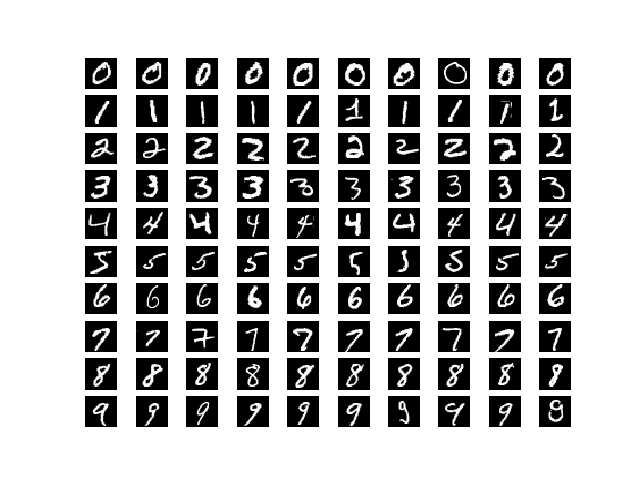
\includegraphics[scale=1]{figures/part1.png}
    \caption{Images from the MNIST dataset}
    \label{fig:fig1}
\end{figure*}

The image is produced from \texttt{plot\_each\_digit()} in \texttt{plot.py}.\\

\end{homeworkProblem}
\clearpage

%----------------------------------------------------------------------------------------
%   PART 2
%----------------------------------------------------------------------------------------

\begin{homeworkProblem}

\textit{Compute Simple Neural Network}\\

The function for computing simple neural network (no hidden layers) is in \texttt{mnist\_handout.py} and is reproduced here.\\

\begin{python}
def compute_simple_network(x, W, b):
    '''Compute a simple network (with no hidden layers)
    '''
    o = np.dot(W.T, x) + b
    return softmax(o)
\end{python}

\texttt{compute\_simple\_network(x, W, b)} returns the output layer of the neural network.\\

\end{homeworkProblem}
\clearpage

%----------------------------------------------------------------------------------------
%   PART 3
%----------------------------------------------------------------------------------------

\begin{homeworkProblem}

\textit{Cost Function: Sum of negative log-probabilities of all training cases}

\subsection{Part 3(a)}
Compute $\frac {\partial C} {\partial w_{ij}}$ (gradient of cost function with respect to a single weight)\\

For one training case, the cost function is (from slide 6 of One-Hot Encoding Lecture):

\begin{equation}
    C = - \sum_{j} y_{j} log p_{j}
\end{equation}

For $M$ training examples, the cost functions gets modified to:\\
\begin{equation}
    C = - \sum_{m=1}^M \sum_{j} y_{j} log p_{j}
\end{equation}

We also know that (from slide 7 of One-Hot Encoding Lecture), 

\begin{equation}
    p_{i} = \frac {e^{o_i}} {\sum_{j} e^{o_j}}
\end{equation}

The partial derivative will be the following:

\begin{equation}
    \frac {\partial p_i} {\partial o_j} = 
        \begin{cases}
            p_i (1 - p_i) &  i = j \\
            - p_i p_j &  i \ne j \
  \end{cases}
\end{equation}

Computing the cost function with respect to the output:
\begin{equation}
\frac {\partial C} {\partial o_i} = \sum_{j} \frac {\partial C} {\partial p_j}  \frac {\partial p_j} {\partial o_i}
\end{equation}

\begin{equation}
 = \frac {\partial C} {\partial p_i}  \frac {\partial p_i}{\partial o_i} - \sum_{j \ne i} \frac {\partial C} {\partial p_j}  \frac {\partial p_j}{\partial o_i}
\end{equation}

\begin{equation}
 = - y_i (1 - p_i) + \sum_{j \ne i} y_j p_j
\end{equation}

\begin{equation}
 = - y_i + p_i \sum_{j \ne i} y_j 
\end{equation}

\begin{equation}
 =  p_i - y_i 
\end{equation}

Computing the O with respect to weight
\begin{equation}
    o_{i} = \sum_{j} w_{ji} x_{j} + b
\end{equation}

\begin{equation}
    \frac {\partial o_i} {\partial w_{ij}} = \sum_j x_j
\end{equation}


Computing the cost function with respect to the weight
\begin{equation}
    \frac {\partial C} {\partial w_{ij}} =\sum_j \frac {\partial C} {\partial o_i} \frac {\partial o_i} {\partial w_{ij}} 
\end{equation}

we will get 
\begin{equation}
    \frac {\partial C} {\partial w_{ij}} = x_j (p_i - y_i)
\end{equation}

\clearpage

%__________________________________

\subsection{Part 3(b)}

\textbf{Compute Gradient of Cost Function with respect to Weight}\\

The function for computing the gradient with respect to weight is in \texttt{mnist\_handout.py} and is reproduced here.\\

\begin{python}
def gradient_simple_network_w(x, W, b, y):
    p = compute_simple_network(x, W, b)

    p_minus_y = np.subtract(p, y)
    gradient_mat = np.matmul(x, p_minus_y.T)

    return gradient_mat
\end{python}

\textbf{Compute Gradient of Cost Function with respect to Bias}\\

The function for computing the gradient with respect to bias is in \texttt{mnist\_handout.py} and is reproduced here.\\

\begin{python}
def gradient_simple_network_b(x, W, b, y):
    p = compute_simple_network(x, W, b)

    return np.sum((p - y), axis=1).reshape((10, 1))
\end{python}

\textbf{Finite difference check}\\

The gradient with respect to weight at several different coordinates was computed and displayed along with the finite difference values at the same coordinates.\\

As can be seen, the gradient is accurate up to 4-5 decimal places.\\

\begin{verbatim}
Index: 245.0, 9.0
Actual Gradient Value:   0.0508788452877
Finite Difference Value: 0.0508927423062

Index: 241.0, 4.0
Actual Gradient Value:   0.030247790924
Finite Difference Value: 0.030294025573

Index: 686.0, 4.0
Actual Gradient Value:   0.0288074199276
Finite Difference Value: 0.0288493552549

Index: 571.0, 7.0
Actual Gradient Value:   -0.0403508424702
Finite Difference Value: -0.040346477939

Index: 180.0, 3.0
Actual Gradient Value:   -0.0110842325284
Finite Difference Value: -0.0110820650203

Index: 408.0, 6.0
Actual Gradient Value:   0.00594562385543
Finite Difference Value: 0.00595885681642

Index: 216.0, 6.0
Actual Gradient Value:   0.0111480447289
Finite Difference Value: 0.0111945692614
\end{verbatim}

This is done in \texttt{check\_grad\_w(x, W, b, y, h, coords)} in \texttt{mnist\_handout.py}.\\


\end{homeworkProblem}
\clearpage

%----------------------------------------------------------------------------------------
%   PART 4
%----------------------------------------------------------------------------------------

\begin{homeworkProblem}

\textit{Train the neural network using Gradient Descent}\\

The code to train the neural net is included in \texttt{mnist\_handout.py}.\\

\begin{python}
def train_nn(f, df_W, df_b, x_train, y_train, x_test, y_test, init_W, init_b, alpha, max_iter = 2000):
    x = x_train
    y = y_train

    epoch, train_perf, test_perf = [], [], []

    EPS = 1e-10
    prev_W = init_W - 10 * EPS
    prev_b = init_b - 10 * EPS
    W = init_W.copy()
    b = init_b.copy()
    itr = 0

    while norm(W - prev_W) > EPS and norm(b - prev_b) > EPS and itr < max_iter:
        prev_W = W.copy()
        prev_b = b.copy()

        W -= alpha * df_W(x, W, b, y)
        b -= alpha * df_b(x, W, b, y)

        if itr % 500 == 0 or itr == max_iter - 1:
            epoch_i = itr
            train_perf_i = performance(x_train, W, b, y_train)
            test_perf_i = performance(x_test, W, b, y_test)

            epoch.append(epoch_i)
            train_perf.append(train_perf_i)
            test_perf.append(test_perf_i)

            print("Epoch: " + str(epoch_i))
            print("Training Performance:   " + str(train_perf_i) + "%")
            print("Testing Performance:    " + str(test_perf_i) + "%\n")

        itr += 1

    return W, b, epoch, train_perf, test_perf
\end{python}

The following optimization procedue was followed:
\begin{enumerate}
    \item Weights were initialized using the saved weights from \texttt{snapshot50.pkl} file. These performed better than randomly initialized weights. I suspect these are pre-trained weights that give a better starting point than random weights.
    \item Learning rate was set to $1^{-5}$ and iterations to 2000. This was done with experiments and trying to see which combination gave the lowest cost on the testing set.
\end{enumerate}

\clearpage

The performance of the NN on training set is 93.24\% and on the testing set is 92.57\%. This is good for a neural net with no hidden layers on the MNIST dataset according to literature available on the web.\\

Performance of the learning curves can be seen in Figure $2$.

\begin{figure*}[h!]
    \centering
    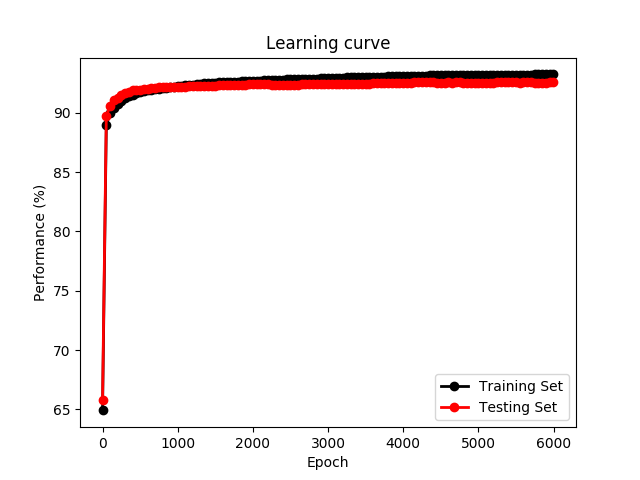
\includegraphics[scale=1]{figures/part4_learning_curve.png}
    \caption{Learning curve for neural network using Gradient Descent}
    \label{fig:fig2}
\end{figure*}

The weights corresponding to each digit are plotted below:\\

\begin{figure*}[h!]
    \centering
    \begin{subfigure}{0.09\textwidth}
        \centering
        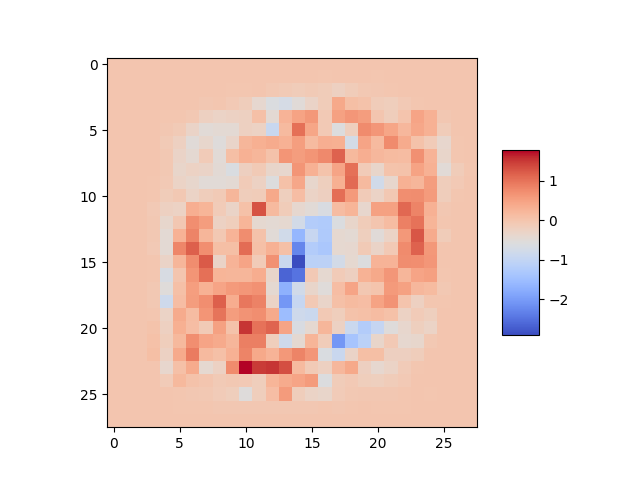
\includegraphics[scale=0.09]{figures/part4_0.png}
        \caption{0}
        \label{fig:sfig1}
    \end{subfigure}
    \begin{subfigure}{0.09\textwidth}
        \centering
        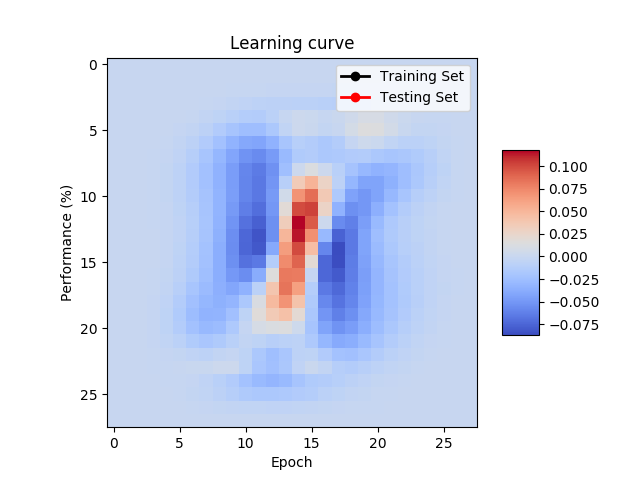
\includegraphics[scale=0.09]{figures/part4_1.png}
        \caption{1}
        \label{fig:sfig1}
    \end{subfigure}
    \begin{subfigure}{0.09\textwidth}
        \centering
        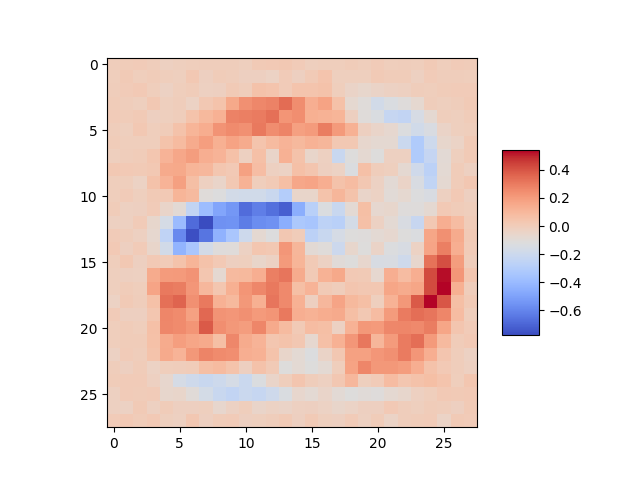
\includegraphics[scale=0.09]{figures/part4_2.png}
        \caption{2}
        \label{fig:sfig1}
    \end{subfigure}
    \begin{subfigure}{0.09\textwidth}
        \centering
        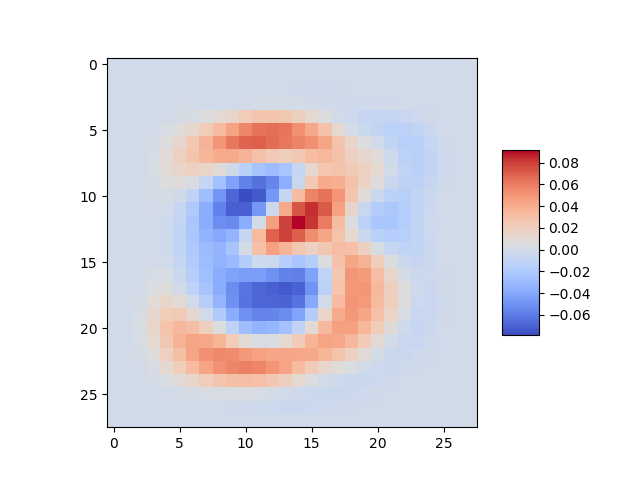
\includegraphics[scale=0.09]{figures/part4_3.png}
        \caption{3}
        \label{fig:sfig1}
    \end{subfigure}
    \begin{subfigure}{0.09\textwidth}
        \centering
        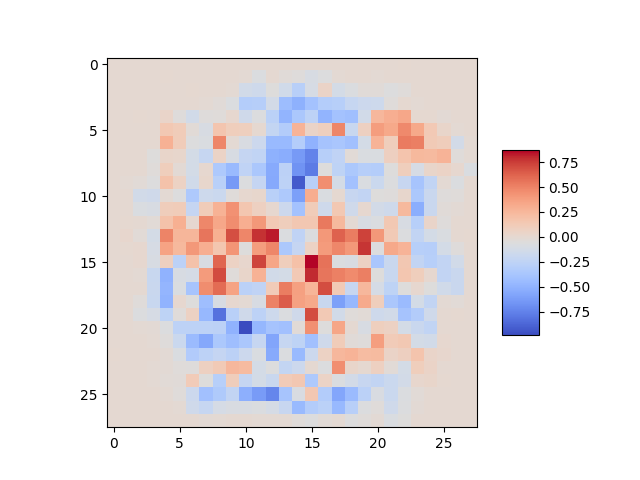
\includegraphics[scale=0.09]{figures/part4_4.png}
        \caption{4}
        \label{fig:sfig1}
    \end{subfigure}
    \begin{subfigure}{0.09\textwidth}
        \centering
        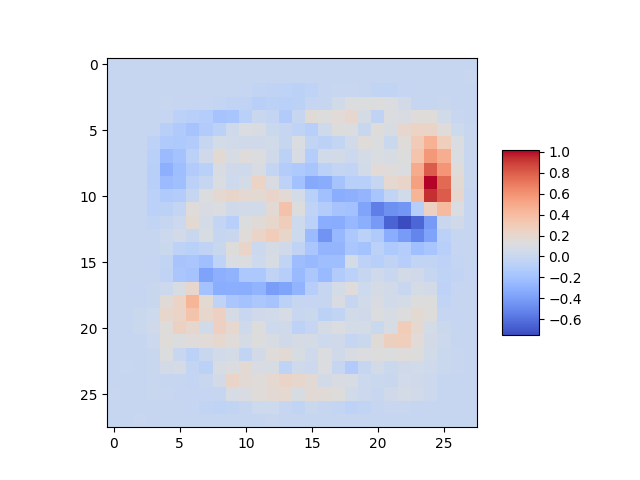
\includegraphics[scale=0.09]{figures/part4_5.png}
        \caption{5}
        \label{fig:sfig1}
    \end{subfigure}
    \begin{subfigure}{0.09\textwidth}
        \centering
        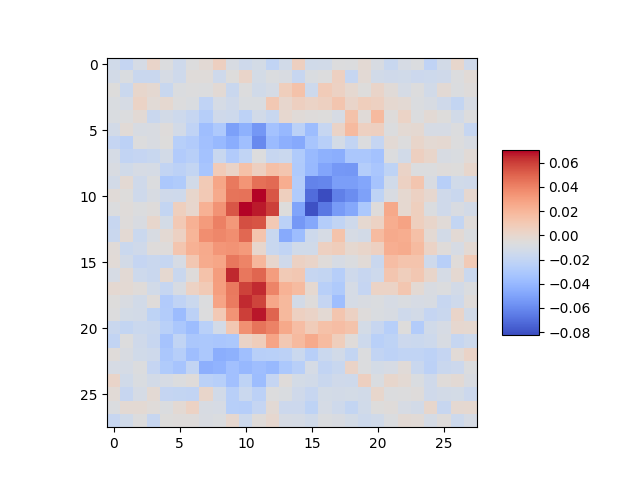
\includegraphics[scale=0.09]{figures/part4_6.png}
        \caption{6}
        \label{fig:sfig1}
    \end{subfigure}
    \begin{subfigure}{0.09\textwidth}
        \centering
        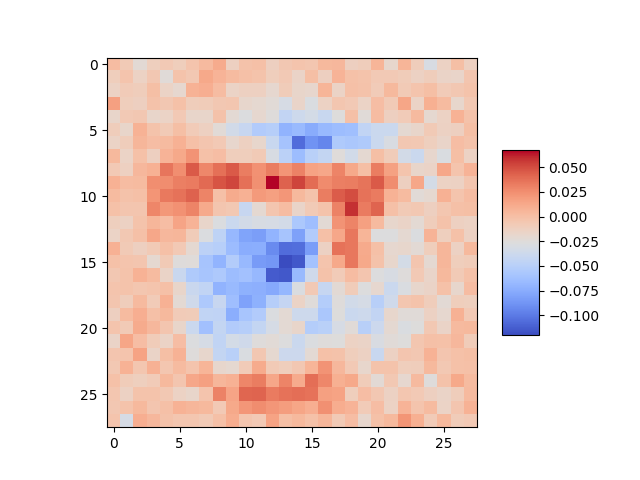
\includegraphics[scale=0.09]{figures/part4_7.png}
        \caption{7}
        \label{fig:sfig1}
    \end{subfigure}
    \begin{subfigure}{0.09\textwidth}
        \centering
        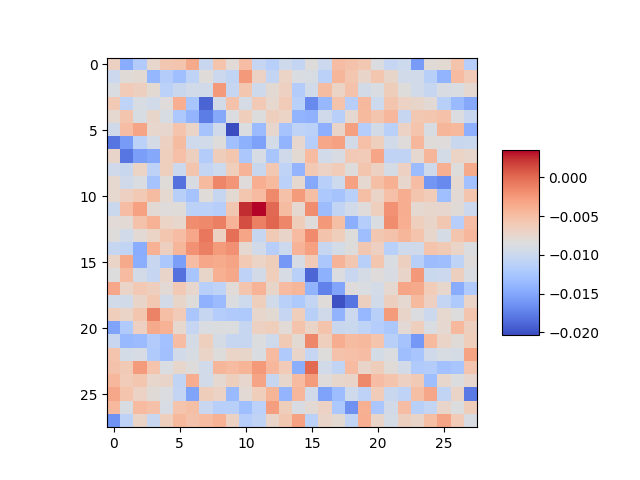
\includegraphics[scale=0.09]{figures/part4_8.png}
        \caption{8}
        \label{fig:sfig1}
    \end{subfigure}
    \begin{subfigure}{0.09\textwidth}
        \centering
        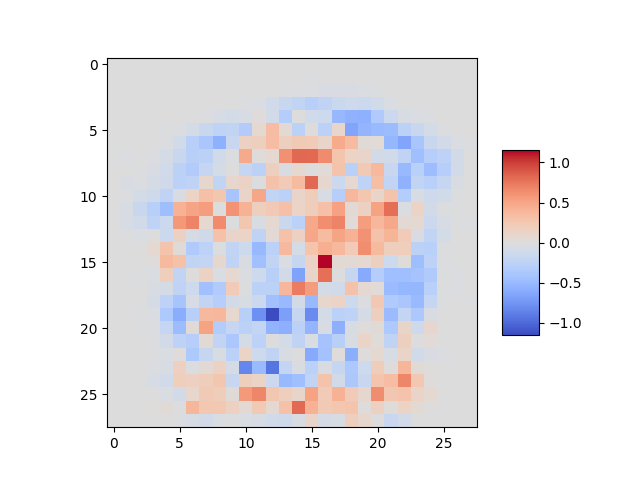
\includegraphics[scale=0.09]{figures/part4_9.png}
        \caption{9}
        \label{fig:sfig1}
    \end{subfigure}
    \caption{Displaying weights of each of the digits}
    \label{fig:fig3}
\end{figure*}

The images can be reproduced by calling \texttt{part4()} in \texttt{digits.py}.\\

\end{homeworkProblem}
\clearpage

%----------------------------------------------------------------------------------------
%   PART 5
%----------------------------------------------------------------------------------------

\begin{homeworkProblem}

\textit{Train the neural network using Gradient Descent with Momentum}\\

The code to train the neural net is included in \texttt{mnist\_handout.py}.\\

\begin{python}
def train_nn_M(f, df_W, df_b, x_train, y_train, x_test, y_test, init_W, init_b, alpha, gamma = 0.9, max_iter = 6000):
    x = x_train
    y = y_train

    epoch, train_perf, test_perf = [], [], []

    EPS = 1e-10
    prev_W = init_W - 10 * EPS
    prev_b = init_b - 10 * EPS
    W = init_W.copy()
    b = init_b.copy()
    itr = 0
    v_W = 0
    v_b = 0

    while norm(W - prev_W) > EPS and norm(b - prev_b) > EPS and itr < max_iter:
        prev_W = W.copy()
        prev_b = b.copy()

        #update velocities
        v_W = gamma * v_W + alpha * df_W(x,W,b,y)
        v_b = gamma * v_b + alpha * df_b(x,W,b,y)
        #update parameters with momentum
        W = W - v_W
        b = b - v_b

        if itr % 50 == 0 or itr == max_iter - 1:
            epoch_i = itr
            train_perf_i = performance(x_train, W, b, y_train)
            test_perf_i = performance(x_test, W, b, y_test)

            epoch.append(epoch_i)
            train_perf.append(train_perf_i)
            test_perf.append(test_perf_i)

            print("Epoch: " + str(epoch_i))
            print("Training Performance:   " + str(train_perf_i) + "%")
            print("Testing Performance:    " + str(test_perf_i) + "%\n")

        itr += 1

    return W, b, epoch, train_perf, test_perf
\end{python}

\clearpage

Performance of the learning curves can be seen in Figure $4$.

\begin{figure*}[h!]
    \centering
    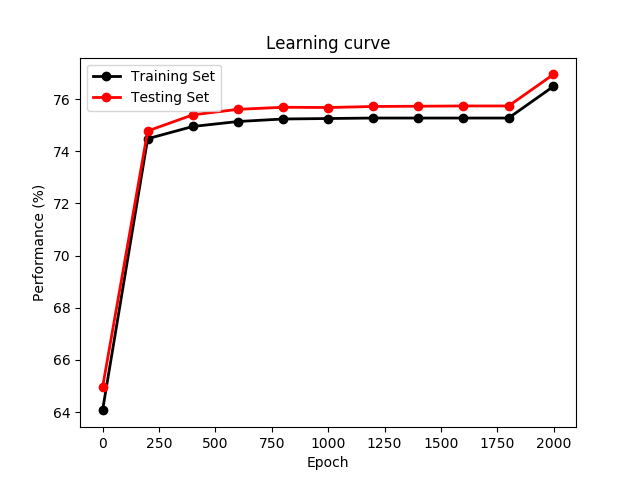
\includegraphics[scale=1]{figures/part5_learning_curve.png}
    \caption{Learning curve for neural network using Gradient Descent with Momentum}
    \label{fig:fig4}
\end{figure*}

It can be observed that with momentum, we reach the peak performance faster than without (notice the steep increase in performance from 0 to 100 iterations). In addition, the performance of the algorithm (in terms of accuracy on the test and training set are not sacrificed). The final performance on the test set was 92.67\% in comparison to 92.57\% by the the training algorithm without momentum.\\

\end{homeworkProblem}
\clearpage

%----------------------------------------------------------------------------------------
%   PART 6
%----------------------------------------------------------------------------------------

\begin{homeworkProblem}

\textit{Gradient descent with momentum}\\

\textbf{Part 6(a)}\\
To choose, $w_{1}$ and $w_{2}$, we looked at the values of the gradient matrix from Part 5, and chose the two gradient indices that had high absolute values.\\

Our aim was to get a plot with a circle in the center but we were not able to get that. We tried different $w_{1}$ and $w_{2}$ and changing the axis for the plot. This part involves a lot of trial and we should have been able to do it had we had more time for experiments.\\

The contour plot is reproduced below:
\begin{figure*}[h!]
    \centering
    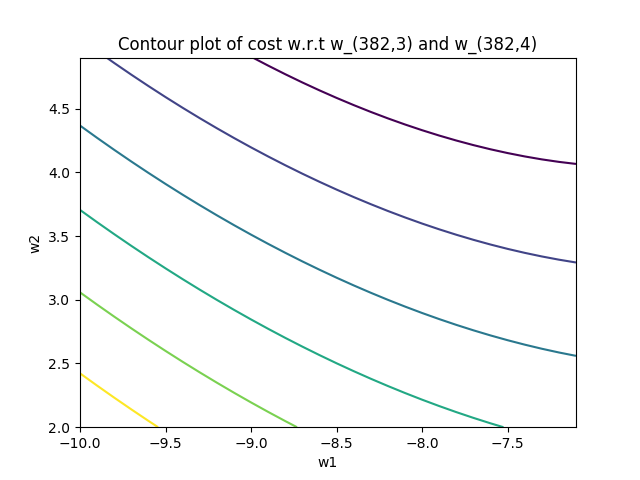
\includegraphics[scale=1]{figures/part6a.png}
    \caption{Contour plot of the cost function}
    \label{fig:fig5}
\end{figure*}

This is done in \texttt{part6a()} in \texttt{digits.py}.\\

\clearpage

\textbf{Part 6(b)}\\

\begin{figure*}[h!]
    \centering
    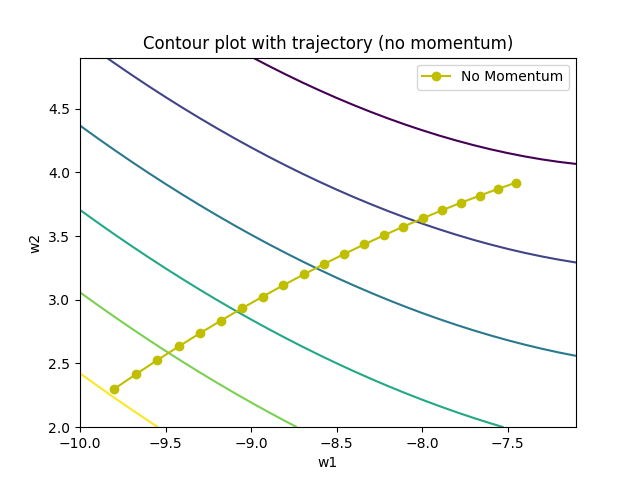
\includegraphics[scale=1]{figures/part6b.png}
    \caption{Trajectory without momentum}
    \label{fig:fig6}
\end{figure*}

Learning rate: $0.01$\\

This is done in \texttt{part6b()} in \texttt{digits.py}.\\

\clearpage

\textbf{Part 6(c)}\\

\begin{figure*}[h!]
    \centering
    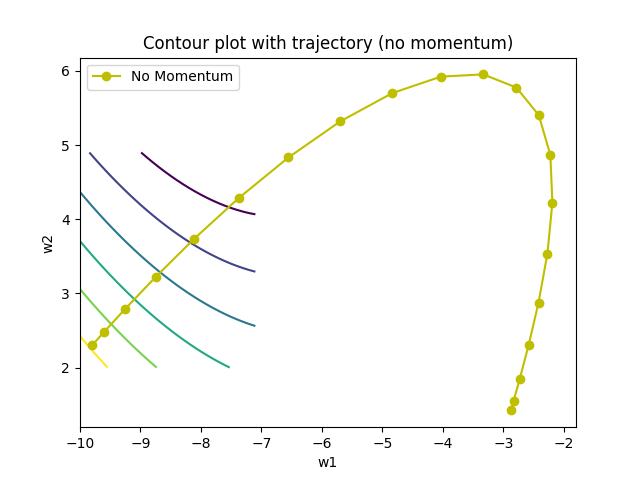
\includegraphics[scale=1]{figures/part6c.png}
    \caption{Trajectory with momentum}
    \label{fig:fig7}
\end{figure*}

Learning rate: $0.01$\\

This is done in \texttt{part6c()} in \texttt{digits.py}.\\

\clearpage

\textbf{Part 6(d)}\\

With momentum, we can see that the weights reach their optimium value in fewer iterations.\\

\clearpage

\textbf{Part 6(e)}\\

I would suspect that for finding cases where momentum is useful, it's important that the particular weight carries a lot of importance in the calculation of the gradient. We tried to do that in Part 6(a) by looking for indices with maximum gradient values. These typically lie in the middle region of the image and where image weights change a lot from image to image.\\

\end{homeworkProblem}
\clearpage

%----------------------------------------------------------------------------------------
%   PART 7
%----------------------------------------------------------------------------------------

\begin{homeworkProblem}

\textit{Backpropogation vs computing the gradient with respect to each weight individually}\\

In this case, we are considering a general, fully-connected neural network with $N$ layers (inclusive of the input and the output layer) each of which contains $K$ neurons.\\

We assume that multiplication of two square matrices is a cubic time complexity operation with respect to the size of the matrix and that the forward pass is cached.\\

\textbf{Computing gradient with respect to each weight term individually}\\

The change in cost, $C$ if a weight $W_{(l, j, i)}$ in layer $l$ gets changed is:

\begin{align*}
    \frac {\partial C} {\partial W_{(l, j, i)}} = \sum_{j^{(N)}=1}^K \frac {\partial C} {\partial h_{(N, j^{(N))}}} \frac {\partial h_{(N, j^{(N))}}} {\partial W_{(l, j, i)}}
\end{align*}

And further, $\frac {\partial h_{(N, j^{(N))}}} {\partial W_{(l, j, i)}}$ depends on layers lower down in the network.

\begin{align*}
    \frac {\partial h_{(N, j^{(N))}}} {\partial W_{(l, j, i)}} =& \sum_{j^{(N-1)}=1}^K \frac {\partial h_{(N, j^{(N))}}} {\partial h_{(N-1, j^{(N-1))}}} \frac {\partial h_{(N-1, j^{(N-1))}}} {\partial W_{(l, j, i)}}\\
    \frac {\partial h_{(N-1, j^{(N-1))}}} {\partial W_{(l, j, i)}} =& \sum_{j^{(N-2)}=1}^K \frac {\partial h_{(N-1, j^{(N-1))}}} {\partial h_{(N-2, j^{(N-2))}}} \frac {\partial h_{(N-2, j^{(N-2))}}} {\partial W_{(l, j, i)}}\\
    \vdots&\\
    \frac {\partial h_{(l+1, j^{(l+1))}}} {\partial W_{(l, j, i)}} =& \sum_{j^{(l)}=1}^K \frac {\partial h_{(l+1, j^{(l+1))}}} {\partial h_{(l, j^{(l))}}} \frac {\partial h_{(l, j^{(l))}}} {\partial W_{(l, j, i)}}\\
\end{align*}

In addition to the changes incurred along the layers, each change in parameter affects each node it connects to in the next layer (as the network is fully connected). In essence, each change in weight value \textit{branches} off $K$ times in the next layer. For an $N$ layer neural network, this means $K^N$ repetitions for each change in the bottom-most layer's weights.\\

Thus, the total cost for gradient computation is:\\

\begin{align*}
    \sum_{(l, j, i)} C_{W_{(l, j, i)}} &= N K^N + N K^{N-1} + \hdots + N K \\
    &= N \frac {1 - K^{N+1}} {1 - K} \\
    &= O(N K^N)
\end{align*}

\clearpage

\textbf{Computing gradient using backpropogation}\\

With (fully vectorized) backpropogation, we are essentially multilpying two 2-Dimensional matrices when we have to compute the gradient for each layer.\\

Since each layer has $K$ neurons and there are $N$ layers in total, this makes the cost to be $O(N K^3)$, since multiplying two matrices is a cubic time complexity operation.\\

Thus, we can observe that backpropogation is a much faster procedure for computing gradient than computing gradient with respect to each weight individually.\\

\end{homeworkProblem}
\clearpage

%----------------------------------------------------------------------------------------
%   PART 8
%----------------------------------------------------------------------------------------

\begin{homeworkProblem}

\textit{Using PyTorch for FaceScrub face classification}\\

\textbf{Architecture of the system}\\
\begin{enumerate}
    \item \textbf{Training and testing set:} Testing set includes 20 images from each actor. The rest of the images for each actor is in the testing set.
    \item \textbf{Getting images:} Used \texttt{get\_and\_crop\_images(act, 64)} and \texttt{remove\_bad\_images(64)} in \texttt{faces.py} to get RGB images of actors and crop them into 64x64 RGB images. Images were checked for SHA-256 checksums and bad images were hardcoded and removed programatically. Using 64x64 RGB images performed better than using 32x32 or grayscale images.
    \item \textbf{Preprocessing the images:} Images were normalized into [-1, 1] and reshaped into vectors of shape (1, 64*64*3)
    \item \textbf{Number of hidden neurons:} Used 600 neurons in one hidden layer. The number of neurons were increased until they were not bringing the cost down for corresponding epochs (perhaps due to overfitting). Increasing number of hidden layers did not give any significant increase in performance.
    \item \textbf{Activation Function:} Used ReLU for the hidden layer activation function. ReLU gave better performace than Tanh or Sigmoid.
    \item \textbf{Mini Batches:} Training was done in batches of 20 random images each. It was made sure that each batch would have a different set of images for training than others. However, the batches themselves repeat after 30 iterations as there are only 600 images while there are 700 iterations to get the best performance.
    \item \textbf{Gradient Optimizer:} Used Adam optimizer. Other optimizers were tried (SGD, AdaGrad) but Adam gave the best performance.
    \item \textbf{Learning rate and max iterations:}Used learning rate of $1^{-4}$ and 700 iterations. Using more iterations increased cost (due to overfitting). The learning rate was low enough to achieve good performance while not having a lot of iterations.
\end{enumerate}

The model, training, and performance is in \texttt{part8()} of \texttt{deepfaces.py}.\\

The final performace of the system was 99.833\% on the training set and 83.33\% on the test set. This is substantially better than the 72\% testing performance achieved on the linear regression model in Project 1.\\

The performance curve is shown in Figure 8.\\

\clearpage

\textbf{Performance curve}\\
\begin{figure*}[h!]
    \centering
    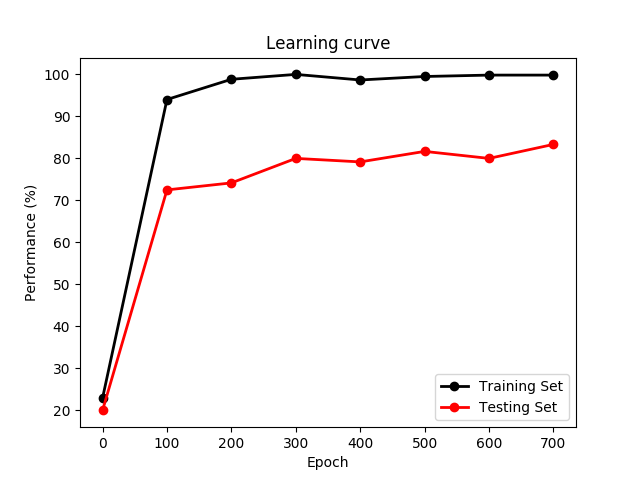
\includegraphics[scale=1]{figures/part8_learning_curve.png}
    \caption{Learning curve for the PyTorch neural network}
    \label{fig:fig8}
\end{figure*}

\end{homeworkProblem}
\clearpage

%----------------------------------------------------------------------------------------
%   PART 9
%----------------------------------------------------------------------------------------

\begin{homeworkProblem}

\textit{Visualizing weights for the hidden unit for two actors}\\

This is done in \texttt{part9()} of \texttt{deepfaces.py}.\\

To select hidden units that are useful for classifying input photos as those particular actors, I ran an image of each actor through the first layer of the neural net made in Part 8 and extracted the indices of the top 10 hidden neurons (according to the highest value of the activation values after taking a softmax of them all). Since, the activation function is ReLU, all the values of the hidden neuron activations is positive and a higher value indicates that it is contributing more to the final outcome.\\

We used the images \texttt{cropped64/bracco27.jpg} and \texttt{cropped64/baldwin38.jpg} respectively for the actors, Bracco and Baldwin. Out of the 10 images generated for each actor, I've picked two that resemble faces the most. All the images can be found in \texttt{figures/bracco} and \texttt{figures/baldwin}.\\

\begin{figure*}[h!]
    \centering
    \begin{subfigure}{0.49\textwidth}
        \centering
        
\includegraphics[scale=2.5]{figures/bracco/part9_bracco_4.jpg}
        \caption{part9\_bracco\_4.jpg}
        \label{fig:sfig1}
    \end{subfigure}
    \begin{subfigure}{0.49\textwidth}
        \centering
        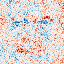
\includegraphics[scale=2.5]{figures/baldwin/part9_baldwin_3.jpg}
        \caption{part9\_baldwin\_3.jpg}
        \label{fig:sfig1}
    \end{subfigure}
    \caption{Visualizing weights of hidden units for classifying images as Bracco and Baldwin}
    \label{fig:fig9}
\end{figure*} 

The images roughly resemble faces (eyes, eyebrows and mouth can be made out). The images do seem a bit noisy which might be due to the fact that the R, G and B layers have been combined to make this image or it might be due to overfitting.\\ 

\end{homeworkProblem}
\clearpage

%----------------------------------------------------------------------------------------
%   PART 10
%----------------------------------------------------------------------------------------

\begin{homeworkProblem}

\textit{Note: The NN's forward method does not work on wolf.teach.cs due to RAM limitations but works on the physical lab machine where it was developed}\\

\textit{Modify AlexNet for FaceScrub face classification}\\

\textbf{Extracting activation values from MyAlexNet}\\

The values of activation of the AlexNet Conv4 layer were extracted by modifying the features of \texttt{MyAlexNet}. We chose Conv4 as it the convolutional layer closest to the output and thus is more likely to have high-level features better for detecting faces.
\begin{enumerate}
    \item Features after Conv4 layer were commented out
    \item Classifer call was removed in \texttt{forward(x)} method so that it returns the activation values instead of classification output
\end{enumerate}

Final (modified) code for \texttt{MyAlexNet} is reproduced here.
\begin{python}
class MyAlexNet(nn.Module):
    def load_weights(self):
        an_builtin = torchvision.models.alexnet(pretrained=True)
        
        features_weight_i = [0, 3, 6, 8, 10]
        for i in features_weight_i:
            self.features[i].weight = an_builtin.features[i].weight
            self.features[i].bias = an_builtin.features[i].bias
            
        classifier_weight_i = [1, 4, 6]
        for i in classifier_weight_i:
            self.classifier[i].weight = an_builtin.classifier[i].weight
            self.classifier[i].bias = an_builtin.classifier[i].bias

    def __init__(self, num_classes=1000):
        super(MyAlexNet, self).__init__()
        self.features = nn.Sequential(
            nn.Conv2d(3, 64, kernel_size=11, stride=4, padding=2),
            nn.ReLU(inplace=True),
            nn.MaxPool2d(kernel_size=3, stride=2),
            nn.Conv2d(64, 192, kernel_size=5, padding=2),
            nn.ReLU(inplace=True),
            nn.MaxPool2d(kernel_size=3, stride=2),
            nn.Conv2d(192, 384, kernel_size=3, padding=1),
            nn.ReLU(inplace=True),
            nn.Conv2d(384, 256, kernel_size=3, padding=1),
            nn.ReLU(inplace=True),
            nn.Conv2d(256, 256, kernel_size=3, padding=1)
            #nn.ReLU(inplace=True),
            #nn.MaxPool2d(kernel_size=3, stride=2),
        )
        self.classifier = nn.Sequential(
            nn.Dropout(),
            nn.Linear(256 * 6 * 6, 4096),
            nn.ReLU(inplace=True),
            nn.Dropout(),
            nn.Linear(4096, 4096),
            nn.ReLU(inplace=True),
            nn.Linear(4096, num_classes),
        )
        
        self.load_weights()

    def forward(self, x):
        x = self.features(x)
        x = x.view(x.size(0), 256 * 13 * 13)
        # x = self.classifier(x)
        return x
\end{python}
This code can be found in \texttt{myalexnet.py}\\

The activation value for an image can be found out by calling \texttt{model.forward(x)} and storing it in a \texttt{numpy} array.
\begin{python}
x = Variable(torch.from_numpy(img), requires_grad=False).type(torch.FloatTensor)
activation = model.forward(x).data.numpy()
\end{python}
The image array is formed by loading in an RGB image of dimensions 227x227, normalizing the values to be in range [-1, 1] and reshaping it in array of shape (1, 3, 227, 227).\\

\textbf{Getting activations for train and test set}\\

Similar to Part 8, each actor has 20 images in test set and the rest in training set. The train-test split is in \texttt{build\_sets\_part10(actor)} in \texttt{faces.py}.\\ 

The images are obtained from the FaceScrub dataset using the function, \texttt{get\_and\_crop\_images(act, 227)} in \texttt{faces.py}. The images are checked for SHA-256 checksums and remaining bad images are filtered out using \texttt{remove\_bad\_images(227)}.\\

\textit{Note: The images are stored in cropped227/ folder which can be obtained by unzipping cropped227.zip. Alternatively, comment out the lines in part10() that call for get\_and\_crop\_images(act, 227) and remove\_bad\_images(227)}\\

The activations for each image is obtained and stored in \texttt{train\_activation} and \texttt{test\_activation} \texttt{numpy} arrays respectively. This is done in \texttt{alexNetFaceScrub()} in \texttt{myalexnet.py}. The process is done 100 images at a time due to CDF machine's memory constraints and will have to be modified should there be more than 600 images in the training set or more than 120 in the test set.\\

\textbf{Plugging the activations into the new neural net}\\

Once we have the activation values, we plug them into a neural net which is similar to the one used in Part 8 except the input dimension has been modified to fit the activation layer size.\\

Similar to part 8, the parameters used to gain better performance were:
\begin{enumerate}
    \item Using ReLU for the hidden layer activation function. ReLU gave better performace than Tanh or Sigmoid.
    \item Using 600 neurons in the hidden layer. The number of neurons were increased until they were not bringing the cost down for corresponding epochs (perhaps due to overfitting).
    \item Using Adam optimizer. Other optimizers were tried (SGD, AdaGrad) but Adam gave the best performance.
    \item Using learning rate of $1^{-4}$ and 150 iterations. Using more iterations increased cost (due to overfitting). The learning rate was low enough to achieve good performance while not having a lot of iterations.
\end{enumerate}

The labels were stored as one-hot encoding for the actors. The new neural net is in \texttt{alexNetFaceScrub()} in \texttt{myalexnet.py}.\\

\textbf{Performance}\\

The final model had a 92.5\% accuracy on the test set. This cut down the error rate in Part 8 by more than 50\%. The performance of the model on training and testing set along with the epochs is shown here.\\

\begin{verbatim}
Epoch: 0
Training Set Performance: 33.8870431894%
Testing Set Performance:  28.3333333333%

Epoch: 10
Training Set Performance: 55.1495016611%
Testing Set Performance:  39.1666666667%

Epoch: 20
Training Set Performance: 79.7342192691%
Testing Set Performance:  72.5%

Epoch: 30
Training Set Performance: 91.0299003322%
Testing Set Performance:  80.8333333333%

Epoch: 40
Training Set Performance: 94.6843853821%
Testing Set Performance:  80.0%

Epoch: 50
Training Set Performance: 97.342192691%
Testing Set Performance:  86.6666666667%

Epoch: 60
Training Set Performance: 99.0033222591%
Testing Set Performance:  89.1666666667%

Epoch: 70
Training Set Performance: 99.8338870432%
Testing Set Performance:  89.1666666667%

Epoch: 80
Training Set Performance: 99.8338870432%
Testing Set Performance:  91.6666666667%

Epoch: 90
Training Set Performance: 100.0%
Testing Set Performance:  90.0%

Epoch: 100
Training Set Performance: 100.0%
Testing Set Performance:  90.8333333333%

Epoch: 110
Training Set Performance: 100.0%
Testing Set Performance:  91.6666666667%

Epoch: 120
Training Set Performance: 100.0%
Testing Set Performance:  91.6666666667%

Epoch: 130
Training Set Performance: 100.0%
Testing Set Performance:  91.6666666667%

Epoch: 140
Training Set Performance: 100.0%
Testing Set Performance:  92.5%

Epoch: 149
Training Set Performance: 100.0%
Testing Set Performance:  92.5%
\end{verbatim}

\end{homeworkProblem}
\clearpage

%----------------------------------------------------------------------------------------

\end{document}